\begin{figure}
  \centering
  \begin{tikzpicture}
    \draw[very thick, ->] (0,0) -- (3.8,0) node[anchor=north] {x};
    \draw[very thick, ->] (0,0) -- (0,3.3) node[anchor=east] {y};
    \node at (-0.2,0) {0};
    \node at (0,-0.2) {0};
    \draw[dark-green, local bounding box=rect, very thick]
      (0.2, 0.2) rectangle (3.7, 3.2);
    \node[dark-green]
      at ({$(rect.west)!0.5!(rect.east)$} |- {$(rect.south)!0.9!(rect.north)$}) {New System};
    % first system
    \draw[red, local bounding box=S1, dashed, thick]
      (1.2,0.2) rectangle (3.7,2.7);
    \node[red]
      at ({$(S1.west)!0.35!(S1.east)$} |- {$(S1.south)!0.2!(S1.north)$}) {System1};
    % second system
    \draw[blue, local bounding box=S2, dashed, thick]
      (0.2,1.2) rectangle (3.2,3.2);
    \node[blue]
      at ({$(S2.west)!0.7!(S2.east)$} |- {$(S2.south)!0.2!(S2.north)$}) {System2};
  \end{tikzpicture}
  \hspace{30pt}
  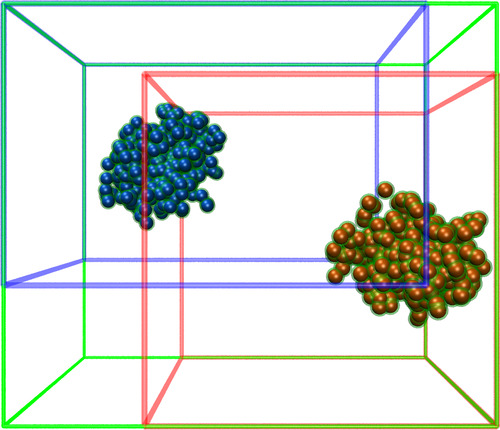
\includegraphics[scale=0.6]{JoinSystems-fig_b.jpg}
  \caption{
    When using no options, the systems are simply put into one file with the new
    box encompassing both the original boxes and bead coordinates unchanged (in
    snapshot, transparent green balls of the new system lie on top of the red
    and blue ones from the original ones).
  }
\end{figure}
